\section*{Appendix}
\addcontentsline{toc}{section}{Appendix}

{ \bf Estimation of Yield Curve with Nelson-Siegel-Svensson Model}

\noindent In their seminal paper, \citet{nelson1987parsimonious} specifies the forward rate curve $\tau(f)$ as follows:

\begin{equation}\notag
    f(\tau)=
    \begin{pmatrix}
    \beta_0 \\ \beta_1 \\ \beta_2    
    \end{pmatrix}'
    \begin{pmatrix}
        1 \\ e^{-\tau/\lambda} \\ (\tau / \lambda) e^{-\tau/\lambda}
    \end{pmatrix}
    =
    \begin{pmatrix}
    \beta_0 \\ \beta_1 \\ \beta_2   
    \end{pmatrix}'
    \begin{pmatrix}
    f_0 \\ f_1 \\ f_2  
    \end{pmatrix}
\end{equation}


% Ridge reg paper'ından aynen aldım
\noindent The spot rate function, which is the average of the forward rate curve up to time to maturity $\tau$, is defined as:

\begin{equation}\notag
    r(\tau)= \frac{1}{\tau}\int_0^\tau f(u)\,du
\end{equation}

\noindent with continuous compounding. Hence, the corresponding spot rate function at time to maturity $\tau$ reads

\newpage

\noindent { \bf Historical Interest Rates}

\begin{figure}[H]
    \centering
    \caption{Long-Term \textit{Nominal} Interest Rates}
    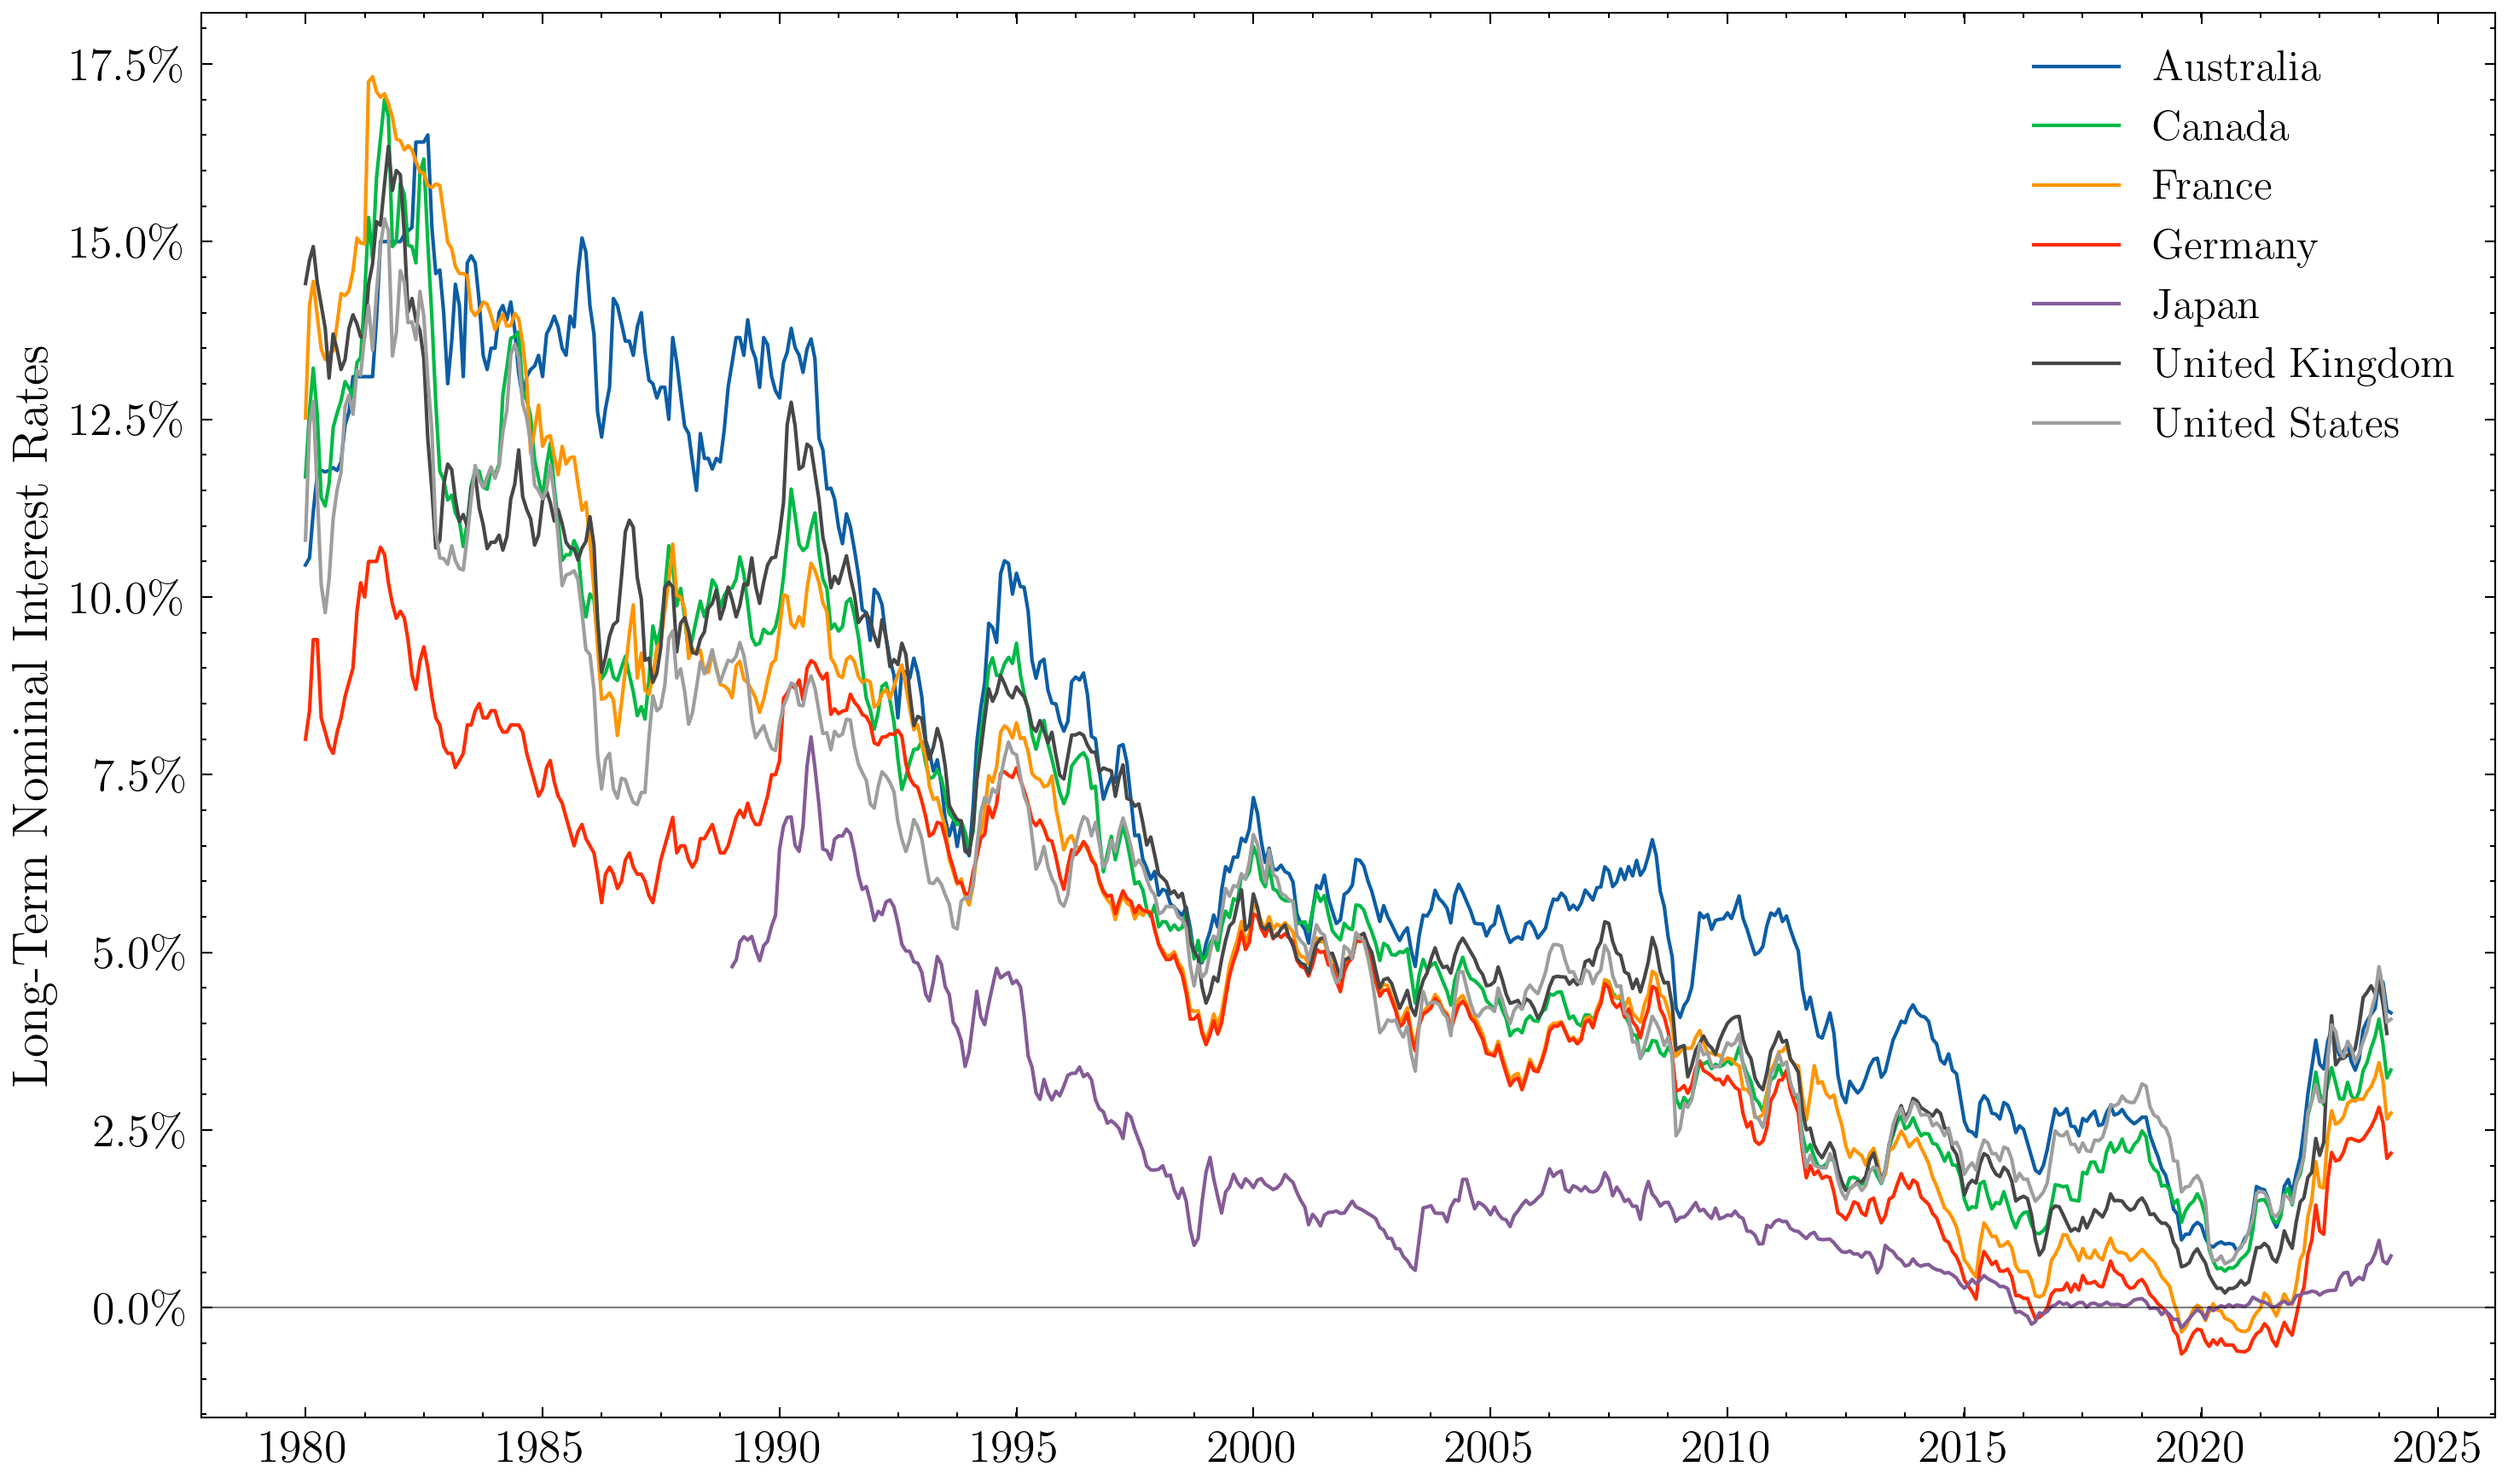
\includegraphics[width=0.8\textwidth]{figures/long-term-rates.png}
    
    \vspace{15pt}
    
    \begin{minipage}{\textwidth}
        \footnotesize % Adjust font size to 8pt
        \textbf{Note:} In this figure, long-term interest rates refer to 10-year bond yields. The data is obtained from OECD Database.
    \end{minipage}
    \label{fig:long-term-rates}
\end{figure}

\begin{figure}[H]
    \centering
    \caption{Yield Curves of Sampled Countries}
    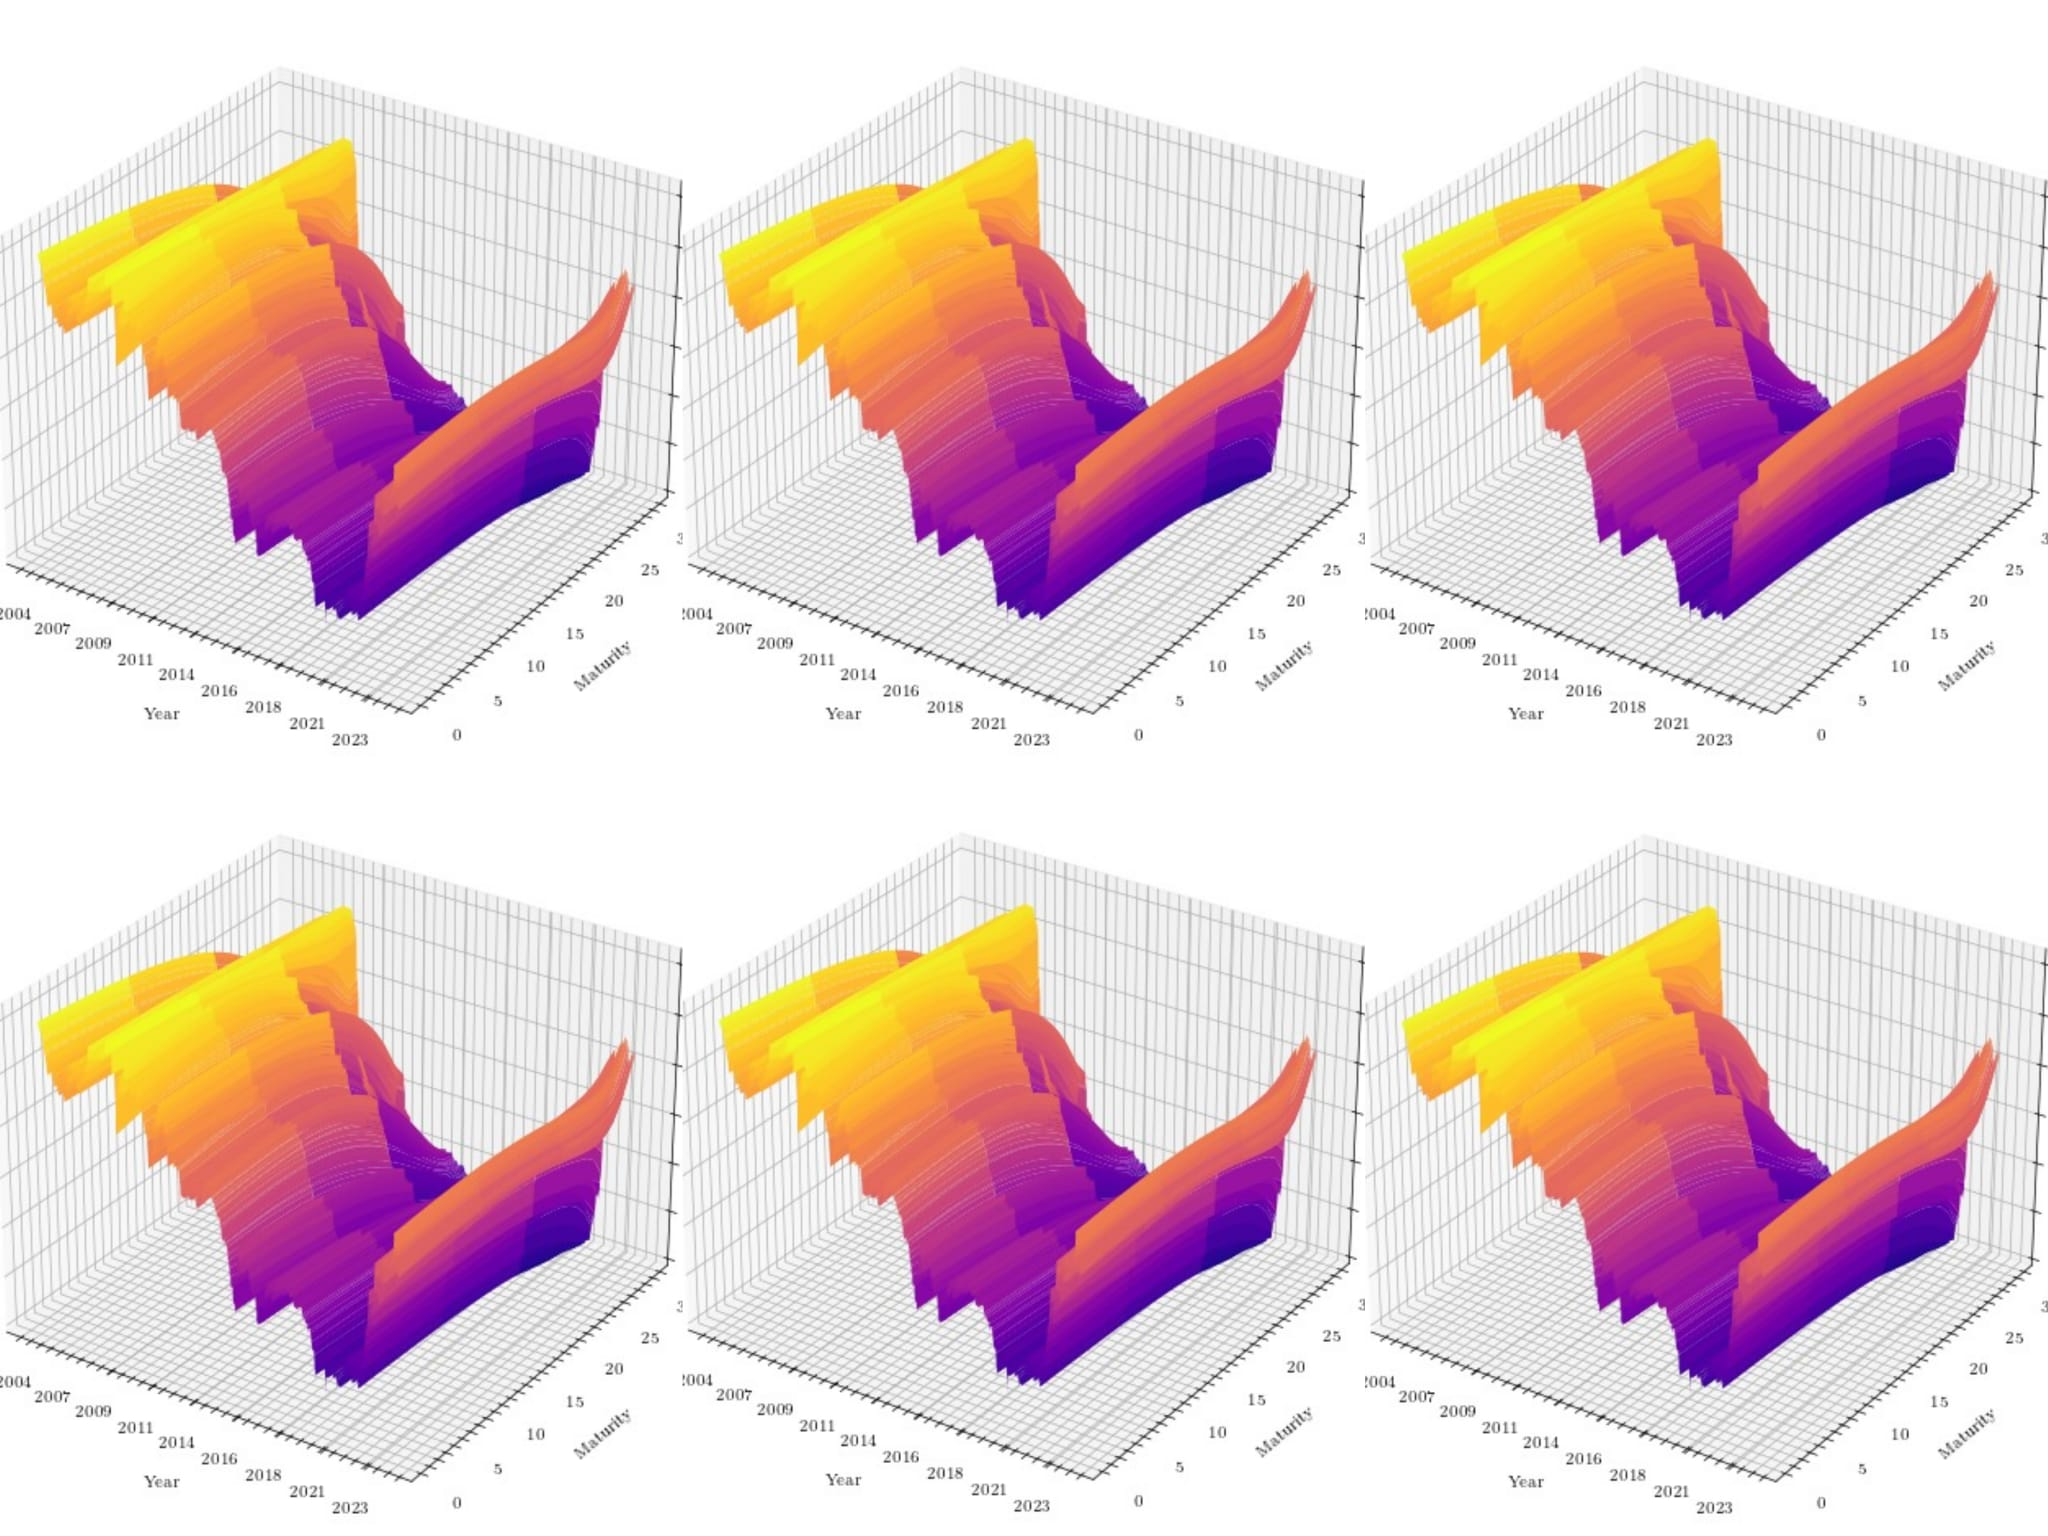
\includegraphics[width=0.9\textwidth]{figures/ycs.jpg}
\end{figure}